%%%%%%%%%%%%%%%%%%%%%%%%%%%%%%%%%%%%%%%%
% Classe do documento
%%%%%%%%%%%%%%%%%%%%%%%%%%%%%%%%%%%%%%%%

% Nós usamos a classe "unb-cic".  Deixe apenas uma das linhas
% abaixo não-comentada, dependendo se você for do bacharelado ou
% da licenciatura.

\documentclass[bacharelado]{unb-cic}
%\documentclass[licenciatura]{unb-cic}



%%%%%%%%%%%%%%%%%%%%%%%%%%%%%%%%%%%%%%%%
% Pacotes importados
%%%%%%%%%%%%%%%%%%%%%%%%%%%%%%%%%%%%%%%%

\usepackage[english]{babel}
\usepackage{acronym}
\usepackage[T1]{fontenc}
\usepackage{indentfirst}
\usepackage{natbib}
\usepackage{mathpartir}
\usepackage{xcolor,graphicx,url}
\usepackage[utf8]{inputenc}
\usepackage{listings, tabularx}
\usepackage{cleveref}
\usepackage{amsmath}
\usepackage{amsthm}
\usepackage{amssymb}
\usepackage{alltt}
\usepackage{xcolor, colortbl}
\usepackage{soul}
\usepackage{wrapfig}
\usepackage{glossaries, cleveref}
\def\MLine#1{\par\hspace*{-\@totalleftmargin}\parbox{\textwidth}{\[#1\]}}


\definecolor{shyellow}{rgb}{.9, .8, .2}
\definecolor{shpurple}{rgb}{.9, .6, .8}

\newcommand{\hlmod}[1]{{%
    \sethlcolor{shyellow}\hl{#1}}%
}

\newcommand{\hlnew}[1]{{%
    \sethlcolor{shpurple}\hl{#1}}%
}


\makeatletter
\newcommand{\displaybump}{\hbox to \@totalleftmargin{\hfil}}
\makeatother

%%%%%%%%%%%%%%%%%%%%%%%%%%%%%%%%%%%%%%%%
% Labels definitions
%%%%%%%%%%%%%%%%%%%%%%%%%%%%%%%%%%%%%%%%
\theoremstyle{definition}
\newtheorem{define}{Definition}[chapter]
\theoremstyle{definition}
\newtheorem{property}{Property}[section]
\newtheorem{theorem}{Theorem}[chapter]
\newtheorem{lemma}{Lemma}[chapter]

%%%%%%%%%%%%%%%%%%%%%%%%%%%%%%%%%%%%%%%%
% lstsliting configurations
%%%%%%%%%%%%%%%%%%%%%%%%%%%%%%%%%%%%%%%%

\lstset{
    breaklines=true,
    postbreak=\raisebox{0ex}[0ex][0ex]{\ensuremath{\color{red}\hookrightarrow\space}}
}



%%%%%%%%%%%%%%%%%%%%%%%%%%%%%%%%%%%%%%%%
% Cores dos links
%%%%%%%%%%%%%%%%%%%%%%%%%%%%%%%%%%%%%%%%

% Veja o arquivos cores.tex se quiser ver que outras cores estão
% pré-definidas.  Utilizando o comando \hypersetup abaixo nós
% evitamos aquelas caixas vermelhas feias em volta dos links.

\input{cores}
\hypersetup{
  colorlinks=true,
  linkcolor=black,
  citecolor=DarkScarletRed,
  filecolor=DarkScarletRed,
  urlcolor= DarkScarletRed
}



%%%%%%%%%%%%%%%%%%%%%%%%%%%%%%%%%%%%%%%%
% Informações sobre a monografia
%%%%%%%%%%%%%%%%%%%%%%%%%%%%%%%%%%%%%%%%

\title{Mechanization and Overhaul of Feature Featherweight Java}

\orientador{\prof \dr Rodrigo Bonifácio de Almeida}{CIC/UnB}
%\coorientador[a]{\prof[a] \dr[a] Coorientadora}{MAT/UnB}
\coordenador{\prof \dr Rodrigo Bonifácio de Almeida}{CIC/UnB}
\diamesano{1}{agosto}{2017}

\membrobanca{\prof \dr Cláudia Nalon}{CIC/UnB}
\membrobanca{Me. Thiago Mael de Castro}{CIC/UnB}

\autor{Pedro da C.}{Abreu Jr.}
%\coautor{Daniella A.}{dos Angelos}
\CDU{004.4}

\palavraschave{Design de Linguagem, Semantica de Linguagem, Java, FOP, Coq}
\keywords{Language Design, Language Semantics, Java, FOP, Coq}



%%%%%%%%%%%%%%%%%%%%%%%%%%%%%%%%%%%%%%%%
% Texto
%%%%%%%%%%%%%%%%%%%%%%%%%%%%%%%%%%%%%%%%


\newacronym{FOP}{FOP}{Feature Oriented Programming}
\newacronym{ITP}{ITP}{Interactive Theorem Prover}
\newacronym{FJ}{FJ}{Featherweight Java}
\newacronym{FFJ}{FFJ}{Feature Featherweight Java}
\newacronym{LFJ}{LFJ}{Lightweight Feature Java}
\newacronym{FM}{FM}{Feature Model}
\newacronym{CA}{CA}{Core Assets}
\newacronym{CK}{CK}{Configuration Knowledge}
% \acrodef{FFJ+}[FFJ\textsubscript{+}]{Overhaul Feature Featherweight Java}
\newacronym{FFJ+}{FFJ$\star$}{Overhaul Feature Featherweight Java}
\newacronym[plural=SPLs]{SPL}{SPL}{Software Product Line}

\makeglossaries
\begin{document}
  \maketitle
  \pretextual

  \begin{dedicatoria}
      Dedico este trabalho ao meu falecido pai Pedro Costa.
      Apesar de sua ausência, sua vida e jornada é uma perene inspiração
      à minha vida.

      E também à minha mãe Rosa Delmira, cuja resiliência,
      bravura e dedicação a iguala aos grandes heróis da antiguidade.
  \end{dedicatoria}

  \begin{agradecimentos}
      No decorrer desta jornada acadêmica alguns personagens chaves cruzaram por ela,
      influenciando profundamente minhas escolhas e meu desenvolvimento pessoal/profissional. Em todo um tempo de vida eu jamais seria capaz de pagar o favor
      que elas fizeram por mim, o melhor que posso fazer é levar no peito a gratidão
      de ter convivido com cada uma delas. Esta é uma lista não exaustiva destas pessoas e alguns de seus ensinamentos.

      Agradeço em primeiro lugar ao meu orientador Rodrigo Bonifácio, figura esta que 
      não cansa de me prover oportunidades de crescimento. Desde os tempos de infância
      acadêmica em POO e LP ele vem me ensinando a sempre buscar por mais e nunca 
      me deixar cair na minha zona de conforto. Agradeço pela oportunidade de trabalhar
      levemente fora de sua área de engenharia de software e me permitir focar em formalização. E acima de tudo por ter feito tudo ao seu alcance para que eu participasse do OPLSS.

      Agradeço ao sesol-4 do TCU, Andrézão, Larissa, Cibele, Maranho, Man Qi, Melgaço,
      Dharlan, Naiara, Felipe, Vinícius, Vitão e Danilo.
      Caso não seja a melhor equipe de TI entre todos órgãos públicos do Brasil,
      certamente é uma das melhores. Todos ali são altamente bem qualificados,
      trabalham duro, e nada menos que padrão Google de qualidade é aceitável.
      Eu tenho a honra não só de dizer que estagiei lá, mas que são meus amigos.
      Agradeço em particular ao meu chefe André Siqueira, que para mim é o modelo vivo de um líder.
      E à Larissa Beatriz, que me recebeu e ensinou como se fosse um filho.

      Agradeço à minha mãe que sempre foi um exemplo vivo de determinação,
      que sempre batalhou por aquilo que acredita, e mais de uma vez se sacrificou
      por mim e meu irmão. Se não fosse por ela eu não estaria onde estou, não somente
      no sentido de ter me provido vida, mas uma boa escola, bons valores e sobretudo
      por nunca ter deixado de acreditar em mim, sempre apoiando minhas decisões, por
      mais difíceis que elas fossem.

      Agradeço ao Ben Lippmeier, por ter sido a razão chave de um excelente estágio
      no NICTA, e também por ter me ensinado tanto apesar de eu não lhe ter provido nenhum retorno palpável. 

      Agradeço aos professores dos departamentos de Ciência da Computação e da Matemática.
      Os professores deste departamento provêm aulas de altíssimo nível,
      permitindo que os alunos se formem tão capacitados quanto em universidades
      de ponta mundo afora.
      Agradeço em especial aos professores: Jorge Lucero, Carla Castanho, Cláudia Nalon, 
      Flávio Moura, Marcos V. Lamar, Bruno Macchiavello, Genaína Nunes, 
      Diego Marques, Lineu Neto, 
      Pedro Roitman e A. Pellegrini. Todos por serem apaixonados pelo que fazem e terem
      me passado um pouquinho desta paixão.

      Agradeço à comunidade do coq no freenode, que foram sempre muito solícitos em
      sanar minhas dúvidas, por mais básicas que fossem.

      Agradeço à Laura Silveira por ter estado ao meu lado por quase metade desta jornada.

      Agradeço aos meus padrinhos João e Márcia, por sempre me fornecer abrigo não apenas em suas casas, mas em seus corações.

      Finalmente agradeço a todos meus amigos e familiares. Zezinho, Paulo, 
      João, Rodrigo, Gaby, Alberto, Laio, Eric, Heloísa, Branco, Dani, Kure, Day, 
      Gaby e Henrique para citar alguns.
  \end{agradecimentos}

  %\begin{resumo}
  %Especificação formal de linguagens vem provado sua eficácia na detecção de
  %possíveis bugs e principalmente no entendimento mais profundo na estrutura da
  %linguagem. Ferramentas de especificação formal e em provas assistida por
  %computadores, como por exemplo Coq, vem sendo alvo de interesse crescente
  %devido à robustez teórica. O objetivo primordial deste trabalho é juntar
  %estas duas frentes e especificar formalmente Feature Featherweight Java em
  %Coq e provar sua corretude.  \end{resumo}

  \begin{abstract}
Specifying a language using an \gls{ITP} is seldom faithful
to its original pen-and-paper specification. However, the process of mechanizing a
language and type safety proofs might also unearth insights for improving the original 
specification. In this work, we detail some design decisions related to our process 
of first specifying \textit{\gls{FJ}} in \texttt{Coq} and thus evolving 
such a specification to prove the type system properties of 
an revised version of \textit{\gls{FFJ}}---a core-calculus for a family of 
languages that address variability management in highly configurable systems, 
such as software product lines (SPLs); which we name as \textit{\gls{FFJ+}}. Indeed, \gls{FFJ+} 
is the first mechanization of \gls{FFJ}, and as such it might also help researchers to 
derive proofs about software product line refinements without considering several 
assumptions about the underlying SPL assets. We believe 
that the whole process led us to a clearer, unambiguous, and equivalent syntax and semantics of 
\gls{FFJ}, while keeping the proofs as well as our \gls{FJ} extensions as simple as possible.

\keywords{Language Design, Language Semantics, Java, FOP, Coq}
\end{abstract}

  \tableofcontents
  \printglossary
  \listoffigures
  \listoftables

  \textual    
  
\chapter{Introduction}
\textit{\gls{FOP}} \cite{prehofer_feature-oriented_1997} is a design methodology and tools for program synthesis \cite{batory_tutorial_2003}.
It aims at the modularization of software systems in terms of features. A \textit{feature}
implements a stakeholder's requirement and is typically an increment in program functionality.
When added to a software system, a feature introduce new structures, such as classes and methods,
and refines existing ones, such as extending methods bodies.

There are several \gls{FOP} languages and tools that provides varying mechanisms
that support the specification and composition of features properly, such as AHEAD \cite{batory_feature-oriented_2004},
FSTComposer \cite{apel_superimposition:_2008}, FeatureC++ \cite{apel_featurec++:_2005}, and more recently Delta-Oriented Programming \cite{schaefer_delta-oriented_2010}. \gls{FOP} has mostly been used to develop
\textit{product-lines} in disparate domains, including compilers for extensible Java dialects 
\cite{batory_jts:_1998}, fire support simulators for U.S. Army \cite{batory_achieving_2000}, high-performance network
\cite{batory_design_1992}, and program verification tools \cite{kurt_stirewalt_component-based_2001}.

Due to the relevance of \gls{FOP}, falar sobre lps...

Several attempts to formalize the type system of \gls{FOP} languages have been made. %Citar todas formalizações de delta oriented programmaning
For instance,  \textit{\gls{FFJ}} \cite{apel_feature_2008} is a proposed type system for \gls{FOP} languages and tools, 
which is developed on top of \textit{\gls{FJ}}~\cite{igarashi_featherweight_2001}
to provide a simple syntax and semantics conforming with common \gls{FOP} languages, 
incorporating constructs for feature composition. %Falar de alguma formalizacao de DOP.

Nevertheless, very few effort was made to mechanize a \gls{FOP} language. In matter of fact, only one
\gls{FOP} language was implemented with a proof assistant to date, it is known as LFJ~\cite{delaware2009machine}
Mechanizing a language is interesting because it makes the proofs even more reliable than peer review.
Take for an instance the Perko Pairs~\cite{little1900xxx}. 
They were listed by C.N Little as different knots in 1885, and only almost a century latter, 
in 1974 Ken Perko discovered~\cite{rolfsen1976knots} them to actually be the same knot!

The idea behind mechanization is to check these proofs with the aid of a computer, reducing significantly the risk of errors, while 
taking full use of automation for the tedious or straightforward steps of the proof. As the system may grow, the mechanization makes
the proof a lot more reliable.

And also, mechanized proofs leads a better organization when the system grows larger.
Better organization of the proof process allows to build teams for these proofs. 
This allows to mechanize correctness properties of big, real world implementations, e.g. compilers~\cite{leroy2012compcert}, 
file systems~\cite{arkoudas2004verifying, amani2015specifying} and languages~\cite{hartel2000formalising, klein2006machine}. 

The process of scrutinizing \gls{FFJ} and defining \textit{unambiguously} its semantics in \texttt{Coq} 
lead us to some language specification and implementation improvements. The biggest change was to review and
simplify the lookup functions of the refinement table.
Henceforth, we refer this proposed calculus as \gls{FFJ+} to distinguish it when comparing our implementation to the original \gls{FFJ} design.
Altogether the improvements proposed in \gls{FFJ+} makes the transition more natural between \gls{FJ} and \gls{FFJ}, 
simplifying the auxiliary functions used in the language specification as well as the type safety proofs and lemmas. 
This allows defining \gls{FFJ+} with incremental changes to \gls{FJ} syntax and semantics, 
and consequently, incremental changes to proofs, leading to a clearer and simpler specification of \textit{FFJ}.


The main goal of this paper is to present a novel mechanization of a \gls{FOP} language. In particular, the mechanization of \gls{FFJ+}.
Hence we can summarize the main contribution of this paper as follows:
\begin{enumerate}
    \item The first mechanization of the \gls{FFJ} type system
    \item An improved specification of \gls{FFJ}, which may help other researchers to reason about software product lines properties.
    \item A report about the benefits of using a proof assistant to revamp an existing specification of a non-mechanized language type system.
\end{enumerate}

This paper is organized as follows: in the Section~\ref{seq:coq} we give a brief introduction to \texttt{Coq} 
Section~\ref{seq:fop} briefly introduces software product lines, \gls{FOP} and \gls{FFJ+},
Section~\ref{seq:offj} gives a brief introduction of  \gls{FFJ+} and explains the main differences with \gls{FJ}
Section~\ref{seq:ffj} formally describes our revamped \gls{FFJ} and states the lemmas needed to preserve \gls{FJ} increment to \gls{FFJ} type safety, 
Section~\ref{seq:impl} discuss the implications of these results to the product line research,
Section~\ref{seq:related} discuss related works and
Section~\ref{seq:conclusion} is the conclusion and shows possible future works.

  \chapter{Theory Fundamentals}\label{chap:theo-fund}
Under the context of software engineering, a lot of effort have been spent in the scope of \textit{reuse}.
However most of the effort have been made code reuse, and not that much into software reuse as a whole.

In this chapter we provide the necessary definitions to understand \gls{FOP},
and how this paradigm copes with software reuse.
To simplify the understanding we will take the examples under software product lines.
This will also make clear how mechanizing a \gls{FOP} language shall benefit real world applications.


\section{Feature Oriented Programming}\label{seq:fop}

Feature-oriented programming (FOP) is a development approach 
that supports the \emph{stepwise refinement strategy} for software 
constructions~\cite{batory-tse2004}. Using FOP, a system is 
typically decomposed in (somewhat new) modular unities 
(named features) that resemble mixing layers~\cite{bracha-ecoop1990}, 
and thus are orthogonal to the typical object-oriented 
decomposition in terms of class hierarchies. 
Successful FOP usage scenarios have been reported in the literature 
for the domains of highly configurable systems and
software product lines~\cite{}.
FOP has been implemented using both programming 
language extensions and tooling support, such as 
Java AHEAD Tool Suite~\cite{batory_feature-oriented_2004} and \textsc{FeatureC++}~\cite{apel_featurec++:_2005}. 


\section{Software Product Line}
In the 70's the concept of software families was introduced by Parnas~\cite{parnas1976design}. 
It's main goal was to enhance the versatility to the development of the artefact's 
non-functional requirements. Upon this, the concept of \gls{SPL}
was formalized with the purpose of projecting several softwares
with similar characteristics under a single domain.

Sommerville~\cite{Sommerville:2010:SE:1841764} defines \gls{SPL} as one of the most effective approaches to reuse.
And defines it as a set of applications with a common architecture and shared components.

As the name suggest, \gls{SPL} idea comes from Ford's product lines. With a product line
it is possible to build several different specializations of the same product, while
improving efficiency and reducing cost. This allow mass individualization of the products, i.e. even though the industry is still delivering products in mass scale,
it still provides somewhat individualized products for different kinds of clients.
The analogue still holds for \gls{SPL}, it proposes a framework which allows to build
several different specializations of the software, 
while reducing delivery time which by its turn reduces cost.

Take for example a \gls{SPL} illustrated in \ref{fig:cellphone-fm} for a mobile phone operational system. 
Every cellphone must be able to make calls and receive calls and having a screen. 
But there are optional features, such as having a GPS, being able to reproduce media,
etc.

\begin{figure}
    \centering
    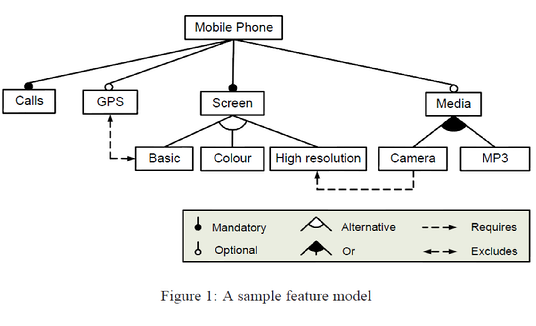
\includegraphics[scale=0.7]{doc/images/mobile-spl}
    \label{fig:cellphone-fm}
    \caption{Cellphone OS feature model} 
\end{figure} 

Formally a \gls{SPL} is defined by a triple: the \gls{FM}, \gls{CA},
and the \gls{CK}.

The \gls{FM} is the set of all features. They may be: \emph{obligatory}, \emph{optional}, \emph{alternative}, \emph{and} and \emph{or}.

The \gls{CA} is everything useful in the process of development, such as documentation, test cases, code, and so on.

The \gls{CK} is a mapping between features to assets, driving product generation.

With that in hand it is possible to compose the assets in order to provide a new product. However, it is not guaranteed that this composition process is safe, i.e.
that every asset selected copes well with each other. This leads us to the safe composition problem.

In order to tackle this safe composition problem, one could manually inspect
\gls{FM}, \gls{CK} and implementation to understand the dependencies between assets for all products. However, since \glspl{SPL} can quickly scale to hundreds of products,
this is often impractical.

Another approach would be to generate every single product, compile and test them.
While this is an useful and safe approach, it does not scale given the exponential 
factor in every feature introduction.

This is where formal methods shines. With formal methods it is possible to study how features interact with each other, postulate properties
and provide safety theorems for \glspl{SPL} without having to generate every single product.

\section{A Running Example: The Expression Product Line in \gls{FOP}}\label{seq:fop-ex}

\begin{wrapfigure}{r}{0.45\textwidth}
    \centering
    \includegraphics[scale=0.35]{doc/images/epl_fm}
    \label{fig:epl_fm}
    \caption{EPL feature model} 
\end{wrapfigure} 


In this section we illustrate the use of FOP through an AHEAD implementation 
of a slight adaptation of the Expression Product Line (EPL)~\cite{torgersen2004expression}---Figure~\ref{fig:epl_fm} shows 
the EPL feature model. Regarding our design decisions, 
in this case we implemented the mandatory features using a \textsc{base} AHEAD package (Figure~\ref{fig:epl-base}), which
declares a class hierarchy involving an interface (\texttt{Expression}) and
several classes (\texttt{Value}, \texttt{BinaryExpression}, \texttt{AddExpression}, and 
\texttt{SubExpression}), and one AHEAD package for each non-mandatory feature (see Figure~\ref{fig:epl-features}). Note 
that an AHEAD package contains either (a) plain Java entities (class or interface) declarations or (b) 
Java entities refinements. A refinement 
might override methods declared in other packages or 
introduce new attributes or methods in existing classes 
or interfaces. In this simple example, we do not implement any 
method overriding through class refinements---the refinements 
only introduce new elements to the \textsc{Base} AHEAD package 
of Figure~\ref{fig:epl-base}.  

\begin{figure}[htb]
    \centering{
        \includegraphics[scale=0.5]{doc/images/base.pdf}
    }
    \label{fig:epl-base}
    \caption{The \textsc{base} package of the Expression Product Line}
\end{figure} 

The details of the EPL AHEAD non-mandatory feature packages are as follows. 

\begin{itemize}
    \item Features \texttt{integer} and {double} refine the \texttt{Value} class of 
    the \textsc{Base} package by introducing a new attribute named 
    \texttt{value}, either with type \texttt{int} or \texttt{double}. According 
    to the EPL feature model, only one of these features might be selected for 
    a given product. 

    \item The \texttt{expressions} feature introduces two new expressions 
    to those declared in the \textsc{Base} package, one for multiplication 
    and another for division. This particular feature does not refine 
    existing classes, only introduces new ones. 

    \item The \texttt{pretty\_printer} feature introduces the support for 
    \emph{pretty printing} expressions. It refines the \texttt{Expression} 
    interface and the \texttt{BinaryExpression} and \texttt{Value} classes, 
    introducing a new method \texttt{print()} and also a 
    new attribute (\texttt{operator}) for the \texttt{BinaryExpression} class.
\end{itemize}


\begin{figure}[htb]
\centering{
\includegraphics[scale=0.5]{doc/images/features.pdf}
}
\label{fig:epl-features}
\caption{Non-mandatory feature implementations of the Expression Product Line}
\end{figure} 


  \chapter{Overview of \gls{FFJ} and \gls{FFJ+}}\label{chap:offj}

\gls{FFJ} is a core calculus for \gls{FOP}, which was built 
upon an extension of \gls{FJ}---a minimal subset of Java. 
In \gls{FFJ}, classes can be added and modified by the 
introduction of a new feature, that is, 
an existing class can be extended by a class refinement. 
A class refinement is declared like a conventional class, though 
preceded by the keyword \texttt{refines}. For example, 
\texttt{refines class C \{$\dots$\}} refers to a class
refinement that
\emph{refines} the class \texttt{C}. The same can be achieved 
for method introduction and modification. Methods refinement,
however, override a previous definition of the corresponding 
method.
 
% \gls{FJ} models a minimal subset of Java. \gls{FFJ} extends \gls{FJ} for \gls{FOP}.
To fully mechanize \gls{FFJ}, we had to disambiguate and enhance 
the language to some extent that it  deserves the attention of 
formally documenting these changes. 
Even though these changes are significant, as discussed in \cref{chap:ffj}, 
the philosophy of \gls{FFJ}, \gls{FOP}, and Stepwise Refinement are maintained.
In \gls{FFJ}, as well as in \gls{FFJ+}, classes can be added and 
modified by the introduction of a new feature.
An existing class can be extended by a class refinement. A class refinement is declared like a class but
preceded by the keyword \texttt{refines}. For example, \texttt{refines class C@feat \{$\dots$\}} refers to a class refinement that
refines the class \texttt{C}. This way, a refinement may add new fields, and methods to the class
and override existing methods.  

A syntactical difference between \gls{FFJ} and \gls{FFJ+} is that, in \gls{FFJ+}, 
the feature notion appears in the abstract syntax tree (AST) of the language.
While the designers of \gls{FFJ} argue that the programmer does not have 
to explicitly state which feature a class or method belongs to, 
we favored the approach of stating the feature in the name of every refinement.
This greatly simplifies the structure of the formalism of the language and can be 
seen as an information gathered by the parser to build the AST, and thus 
the actual code expressed using the concrete syntax of this language 
might not have these annotations.

In addition, an \gls{FFJ+} program has a table with every class 
declaration (\textsf{CT}) and another table with every class refinement (\textsf{RT}).
We make this distinction to simplify the extension from \gls{FJ} in \texttt{Coq}, since 
with this decision we eliminate the need to match whether a class in the table 
is a refination or a declaration. From this \textsf{RT} we can retrieve the composition order
of the refinements and build the refinement chain of the program, 
which is used to check if features were composed correctly and
does not references features that have not been introduced yet. 
We redefine the denotation of \textsf{RT} from \gls{FFJ}.
In the original version, it was used to retrieve the refinement name given a 
refinement declaration. This is no longer necessary in \gls{FFJ+}, since
that information is already encoded in the abstract syntax.

Finally, in the original definition of \gls{FFJ}, the lookup functions are 
somewhat circumvoluted. Accordingly, we propose a very different approach
for them, with the aim as been not only as formal and simple as possible, 
but also easy to evolve from our mechanized version of \gls{FJ}. 
To this end, we eliminate the need for reverse field lookup, reverse method lookup, 
and the refinement relation. A formal description with all these changes 
is given in Section~\ref{subsec:lookup}. Note that, we were only 
able to conceive these improvements while formalizing \gls{FFJ+} in 
\texttt{Coq}. 

In \Cref{lst:expr-ct,lst:expr-rt} we revisit the EPL example from 
\Cref{seq:fop-ex} this time using \gls{FFJ+} instead of AHEAD.

\begin{lstlisting}[language=Java, frame=single, numbers=left, basicstyle=\footnotesize,
    label={lst:expr-ct}, caption={EPL Class Table}, captionpos=b]
class Expr extends Object {
    Expr() { super(); }
}

class Add extends Expr {
    Expr a; Expr b;
    Add(Expr a, Expr b) {super(); this.a=a; this.b=b;}
}

class Sub extends Expr {
    Expr a; Expr b;
    Sub(Expr a, Expr b) {super(); this.a=a; this.b=b;}
}
\end{lstlisting}

\begin{lstlisting}[language=Java, frame=single, numbers=left, basicstyle=\footnotesize,
    label={lst:expr-rt}, caption={EPL Refinement Table}, captionpos=b]
refines class Expr@Eval {
    refines Expr() { original(); }
    int eval() {return 0;}
}

refines class Add@Eval {
    refines Add(Expr a, Expr b){original(a,b);}
    refines int eval() {return this.a.eval() + this.b.eval();}
}


refines class Sub@Eval {
    refines Add(Expr a, Expr b){original(a,b);}
    refines int eval() {return this.a.eval() - this.b.eval();}
}
\end{lstlisting}

Typically, a programmer applies multiple refinements to a class by composing
a sequence of features. The ordered list of refinements is called a \emph{refinement
chain}. The order in which a refinement introduced matters, and a refinement
that is introduced right before another is called \emph{predecessor}. 

As class inheritance, refinements cannot introduce a field with the same
name already declared before. Methods, on the other hand, may overload an already
introduced class, this can be seen in \texttt{Sub@Eval eval} and \texttt{Add@Eval eval}.
Overloading, on the other hand, is not allowed, i.e. if the programmer wants to introduce the
a method with a name that is already used, it must have the same number of arguments, the same argument types
and the same return type as the previous function definition.

The distinction between method introduction and overriding allows the type system to check
if an introduced method inadvertently replaces an existing one with the same name.
The distinction also allows the type system to check if there is proper a method to be overridden.

In order to retrieve the correct fields or the correct method of a class, it is
necessarily to walk in the subclass refinement correctly. As shown in \Cref{fig:refinement-order}
first start from the last refinement of a class, walk through every predecessor,
and when you get to the last refinement, you go to the class, and finally to the
superclass last refinement. And so on until you reach the Object class, which
is the root class of all class hierarchies.

\begin{figure}[htb]
    \centering
    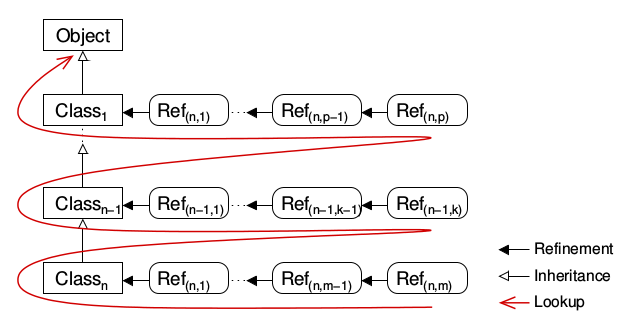
\includegraphics[scale=0.7]{doc/images/refinement-order}
    \label{fig:refinement-order}
    \caption{Order of lookup in \gls{FFJ+}}
\end{figure} 


  \chapter{Overhaul Feature Featherweight Java}\label{seq:ffj}

\section{Syntax}
The Syntax of \gls{FFJ} is a straightforward \gls{FOP} extension of \gls{FJ}. Due to the lack
of space we do not present the formal definition \gls{FJ} nor \gls{FFJ}, but instead we follow
the same scheme of the \gls{FFJ} original definition in \cite{apel_feature_2008} and present
the modified rules from \gls{FFJ} to \gls{FFJ+} highlighted with \hlmod{shaded yellow boxes} 
and new rules highlighted by \hlnew{shaded purple boxes}. Also notice that the successor and 
the refinement relations were simply dropped for being unnecessary by now.

\newcommand{\cdecl}[6]{\texttt{class #1 extends #2 \{\={#3} \={#4}; #5 \={#6}\}}}
\newcommand{\crefine}[6]{\texttt{refines class #1 \{\={#2} \={#3}; #4 \={#5} \={#6}\}}}
\newcommand{\mdecl}[5]{\texttt{#1 #2 (\={#3} \={#4}) \{return #5;\}}}
\newcommand{\mrefine}[5]{\texttt{refines #1 #2 (\={#3} \={#4}) \{return #5;\}}}

\begin{table}[!ht]
    \begin{tabularx}{.62\textwidth}{l|}
        \hlnew{\texttt{R}~::=} \hfill \textit{refinement names:} \\
        \quad \hlnew{\texttt{C@feat}} \\ \\
        \texttt{CD}~::= \hfill \textit{class declarations:}\\
        \quad \cdecl{C}{D}{C}{f}{K}{M} \\  \\
        \hlmod{\texttt{CR}~::=} \hfill \textit{class refinements:}\\
        \quad \hlmod{\texttt{refines class R \{\={C} \={f}; KD \={M} \={MR}\}}} \\ \\
        \texttt{K}~::=  \hfill\textit{constructor declarations:}\\
        \quad \texttt{C(\={C}~\={f})\{super(\={f});~this.\={f}=\={f};\}}\\\\
        \texttt{KD}~::= \hfill\textit{constructor refinements:} \\
        \quad \texttt{refines~C(\={E}~\={h}, \={C} \={f})\{original(\={f}); this.\={f}=\={f};\}} \\\\
        \texttt{M}~::= \hfill\textit{method declarations:}\\
        \quad \mdecl{C}{m}{C}{x}{e}
    \end{tabularx}
    \begin{tabularx}{.4\textwidth}{l}
        \texttt{MR}~::= \hfill \textit{method refinements:}\\
        \quad \mrefine{C}{m}{R}{x}{e} \\ \\
        \texttt{e}~::= \hfill \textit{expressions:}\\
        \quad \texttt{x} \hfill\textit{variable}\\ 
        \quad \texttt{e.f} \hfill\textit{field access}\\
        \quad \texttt{e.m(\={e})} \hfill\textit{method invocation}\\
        \quad \texttt{new~C(\={e})} \hfill\textit{object creation}\\
        \quad \texttt{(C)e} \hfill\textit{cast}\\ \\
        \texttt{v}~::= \hfill \textit{values:}\\
        \quad \texttt{new~C(\={e})} \hfill\textit{object creation}
    \end{tabularx}
    \quad
    \caption{\gls{FFJ} Syntax}
    \label{abstractsyntax}
\end{table}
%\end{center}


The syntax of \gls{FFJ+} constructs is given at \cref{abstractsyntax}. The metavariables
\texttt{A}, \texttt{B}, \texttt{C}, \texttt{D} and \texttt{E} ranges over class names, \texttt{f} and \texttt{g} range over
field names; \texttt{m} ranges method name; \texttt{x} ranges over variable, \texttt{v} ranges over
values, \texttt{feat} ranges over feature names. We assume that the set of variables includes the special variable \texttt{this}, which
cannot be used as the name of an argument of a method.

We write \texttt{\=f} as a shorthand for a possible empty sequence \texttt{f\textsubscript1}, \dots, \texttt{f\textsubscript{n}} 
and similarly for \texttt{\=C}, \texttt{\=x}, \texttt{\=e}, etc. We abbreviate the operations on pairs of sequences
``\texttt{\=C~\=f}'' for ``\texttt{C\textsubscript1~f\textsubscript1},\dots, \texttt{C\textsubscript{n}~f\textsubscript{n}}''
and ``\texttt{this.\=f=\=f;}'' as a shorthand for 
``\texttt{this.\=f\textsubscript1=\=f\textsubscript1;} \dots, \texttt{this.\=f\textsubscript{n}=\=f\textsubscript{n};}''.
We write empty sequence as $\bullet$.


A class declaration \texttt{class\ C~extends~D\ \{\={C} \={f}; K \={M}\}} 
introduces a class \texttt{C} with superclass \texttt{D}. This class has fields \texttt{\=f}
of type \texttt{\=C}, a constructor \texttt{K} and methods \texttt{\=M}. The fields of the class \texttt{C}
is \texttt{\=f} added to the fields of its superclass \texttt{D}, all of them must have distinct names.
Methods, on the other hand, may override another superclass method with the same name.
Method override \gls{FFJ+} is basically method rewriting. 
Methods are uniquely identified by its name, i.e. overloading is not supported.

A class refinement \texttt{refines~class~C@feat~\{\={C}~\={f};~KD~\={M}~\={MR}\}}
introduces a refinement of the class \texttt{C} and belongs to the feature \texttt{feat}. 
This refinement contains the fields  \texttt{\=f} of type \texttt{\=C}, 
a constructor refinement \texttt{KR}, methods declarations \texttt{\=M} and method refinements $\overline{\texttt{MR}}$.
Like class declarations, the fields of a class refinement \texttt{R} are added to the fields of its predecessor, which
is explained in more detail in \Cref{subsec:lookup}.

Constructor declaration \texttt{C(\={C}~\={f})\{super(\={f}); this.\={f}=\={f};\}} and a constructor refinement 
\texttt{refines~C(\={E}~\={h}, \={C}~\={f}) \{original(\={f}); this.\={f}=\={f};\}} introduce a constructor 
for the class \texttt{C} with fields \texttt{\=f} of type \texttt{\=C}. The constructor declaration body is simply 
a list of assignment of the arguments with its correspondent field preceded by calling its superclass constructor with the correspondent arguments.
The constructor refinement only differs from constructor declaration that instead of calling the superclass constructor
it will call its predecessor constructor (denoted by \texttt{original}).

Method declaration \texttt{C~m~(\={C}~\={x})\ \{return~e;\}} and method refinement \texttt{refines C~m~(\={C}~\={x})\ \{return~e;\}} 
introduce a method \texttt{m} of return type \texttt{C} with arguments \texttt{\={C}~\={x}} and body \texttt{e}.
Method declarations can only appear inside a class declarations or refinement, whereas method refinement should only appear
inside a class refinement. There is such a distinction between method declaration and method refinement for allowing the type checker
to recognize the difference between method refinement and inadvertent overriding/replacement.

A class table \textsf{CT} is a mapping from class names \texttt{C} to class declarations \texttt{CD}.
A refinement table \textsf{RT} is a mapping from refinement name \texttt{C@feat} to refinement declarations.
An \gls{FFJ} program consists of a triple (\textsf{CT}, \textsf{RT}, \texttt{e}) of a class table, a refinement table
and an expression. Throughout the rest of the paper the \textsf{CT} and the RT are assumed to be always fixed to lighten the notation.

\section{Lookup Functions}\label{subsec:lookup}

In \gls{FFJ} as well as in \gls{FJ} types are classes and classes have a subclass relation defined by the syntax of class declaration.
To navigate this subclass relation in the \textsf{CT}, the auxiliary operator \texttt{<:} is given in \Cref{table:sub_pred}, this operator is 
the reflexive and transitive closure of the subclass relation.

The \textsf{CT} is expected to satisfy some sanity conditions:
\begin{itemize}
	\item  \textsf{CT}~(\texttt{C}) = \texttt{class C}$\ldots$ for every \texttt{C} $\in$ dom(\textsf{CT})
	\item \texttt{Object} $\notin$ dom(\textsf{CT})
	\item for every class name \texttt{C}~(except \texttt{Object}) appearing anywhere
		in \textsf{CT}, we have \texttt{C} $\in$ dom(\textsf{CT})
	\item there are no cycles in the subtype relation induced by \textsf{CT}, i.e., the
		relation \texttt{<:} is antisymmetric
\end{itemize}

\begin{table}[!ht]

    \raggedright \textit{Subtyping}\\
	\centering
	\begin{tabular}{c@{\qquad}c@{\qquad}c}
		\inferrule{ }{\texttt{C~<:~C}} & 
		\inferrule{\texttt{C <: D} \qquad \texttt{C <: E}}
		{\texttt{C~<:~E}} &
		\inferrule{\texttt{class~C~extends~D~\{~\ldots~\}}}
		{\texttt{C~<:~D}} \\
	\end{tabular}
    \vspace*{2pt}
    \caption{Subtype Relation}
    \label{table:sub_pred}
\end{table}


In \gls{FFJ+} we fetch the refinement precedence via its position in the \textsf{RT}, i.e.
if a refinement of a class appears first in the \textsf{RT} it will be applied first. 
These functions to navigate the \textsf{RT} are all defined in \Cref{table:refinement}
    
First we have the function $class\_name$ which retrieves the name of a class refinement.

Next we define the function $refinements\_of~\texttt{C}$ to retrieve the refinements of 
a given class in the same order as they were introduced in the \textsf{RT}.

To navigate the precedence we define the \textit{pred} and the \textit{last} functions.
The \textit{pred} function will get a class refinement as an argument,
filter refinements of the same class of \texttt{R} as \texttt{\=R}, fetch the $index$ $n$ of \texttt{R} in \texttt{\=R} 
and return the element \texttt{P} at the position $n-1$ in \texttt{\=R} (denoted by the $get$ function). Notice that \textit{pred} is a partial function
because it is not defined if the a refinement is the first refinement.

The \textit{last} function retrieves the last refinement of a given class \texttt{C}.
This is needed because in \gls{FFJ+} we navigate the refinement chain backwards, from the last refinement
to the first, looking for a given method or field. 

\begin{table}[!ht]
	\def\arraystretch{2.5}
    \raggedright \hlnew{\textit{Class Name}}\\
	\centering
    \begin{tabular}{c}
        \rowcolor{shpurple}
        \inferrule{ \texttt{R} = \texttt{C@feat}}
                    {class\_name~\texttt{R} = \texttt{C} }
    \end{tabular}

    \qquad\qquad \\ 
    \raggedright \hlnew{\textit{Refinements of a class}}\\
	\centering
    \begin{tabular}{c}
        \rowcolor{shpurple}
        \inferrule{ filter~(\lambda R \cdot class\_name~\texttt{R} == \texttt{C})~\textsf{RT} = \texttt{\=R}}
                    {refinements\_of~\texttt{C} = \texttt{\=R} }
    \end{tabular}

    \raggedright \hlmod{\textit{Predecessor}}\\
	\centering
    \begin{tabular}{c}
        \rowcolor{shyellow}
        \inferrule{refinements\_of~(class\_name~\texttt{R}) = \texttt{\=R}\\
                  index~\texttt{R}~\texttt{\=R}~=~n\\
                  get~(n-1)~\texttt{\=R}~=~\texttt{P}}
        {\textit{pred}~\texttt{R}~=\texttt{P}}
    \end{tabular}

    \raggedright \hlmod{\textit{Last}}\\
	\centering
    \begin{tabular}{c}
        \rowcolor{shyellow}
        \inferrule{refinements\_of~\texttt{C} = \texttt{\=R}\\
                  tail~\texttt{\=R}~=~\texttt{R}}
        {\textit{last}~\texttt{C}~=\texttt{R}}
    \end{tabular}

    \qquad\qquad
    \caption{Refinement Relations}
    \label{table:refinement}
\end{table}

With this in hand we can define the actual lookup functions $fields$, $mtypes$ and $mbody$.
They are taken directly from \gls{FFJ} definition, with a new hypothesis and an extra rule.
The extra rule and hypothesis makes reference to dealing with the refinements. This is necessary
to make the proofs easier to maintain, since all we need to do is to provide a few acceptance lemmas
about these new lookup functions which we name $fields_R$, $mtype_R$ and $mbody_R$.

$fields_R$ simply retrieves the fields of all refinements up to that point in the refinement chain.

$mtype_R$ and $mbody_R$ tries to find the last introduction to a method, and retrieves its type or body.
These two definitions greatly differs from \gls{FFJ} to \gls{FFJ+}. In \gls{FFJ} $mtype$ would
retrieve the typing of the first method introduction, whereas in \gls{FFJ+} it will retrieve the
type of the last method refinement, and only later we define the rules for guarantying that the
refinement always has the same type of the method declaration. This was made to greatly simplify
the proof that states that if a method has $mtype$ then it also has a $mbody$, since both 
functions follows the same structure the proof is straightforward.


\begin{table}[ht!]
	\centering
	\begin{tabular}{c}
        \rowcolor{shpurple}
        \inferrule{\texttt{refines R \{\=C \=f; KR \=M \={MR}\}} \qquad
                    \neg pred~\texttt{R}}
                {fields_R~\texttt{R}~=~\texttt{\=C \=f}} \\
        \\
        \rowcolor{shpurple}
		\inferrule{\texttt{refines R \{\=C \=f; KR \=M \={MR}\}} \qquad
                    \textit{pred}~\texttt{R}~=~\texttt{P}}
                {fields_R~\texttt{C}=fields_R~\texttt{P, \={C} \={f}}}\\
        \\
	\end{tabular}
	\centering
	\begin{tabular}{c}
		$fields~$\texttt{Object}$=\bullet$ \\
        \\
        \rowcolor{shyellow}
		\inferrule{\texttt{class C extends D \{\=C \=f; K \=M\}} \qquad 
                    \neg\textit{last}~\texttt{C}}
                {fields~\texttt{C}=fields~\texttt{D, \={C} \={f}}} \\
        \\
        \rowcolor{shyellow}
		\inferrule{\texttt{class C extends D \{\=C \=f; K \=M\}} \qquad 
                    \textit{last}~\texttt{C}~=~\texttt{R}}
                {fields~\texttt{C}=fields~\texttt{D, \={C} \={f},} fields_R~\texttt{R}}\\
        \\
	\end{tabular}
    \label{table:field}
    \caption{Field lookup}
\end{table}

\newcommand{\mtype}[2]{\ensuremath{mtype~(\texttt{#1},\texttt{#2})}}
\newcommand{\mtyper}[2]{\ensuremath{mtype_R~(\texttt{#1},\texttt{#2})}}
\newcommand{\mrettype}[2]{\texttt{\={#1}}\ensuremath{~\rightarrow~}\texttt{#2}}

\begin{table}[h!]
	\centering
	\begin{tabular}{c}
        \rowcolor{shpurple}
        \inferrule{\crefine{R}{C}{f}{KR}{M}{MR} \qquad 
                \mdecl{B}{m}{B}{x}{e} \in \texttt{\={M}}}
                {\mtyper{m}{R}~=~\mrettype{B}{B}} \\ 
    \end{tabular}
    \vspace*{.2cm}
    \begin{tabularx}{.55\textwidth}{c}
        \rowcolor{shpurple}
        \inferrule{\crefine{R}{C}{f}{KR}{M}{MR} \qquad 
                \texttt{m} \notin \texttt{\={M}} \\
                \mrefine{B}{m}{B}{x}{e} \in \overline{\texttt{MR}}}
                {\mtyper{m}{R}~=~\mrettype{B}{B}} \\ 
    \end{tabularx}
    \begin{tabularx}{.39\textwidth}{c}
        \rowcolor{shpurple}
        \inferrule{\crefine{R}{C}{f}{KR}{M}{MR} \\\\
                \texttt{m} \notin \texttt{\={M}} \quad
                \texttt{m} \notin \overline{\texttt{MR}} \quad
                pred~\texttt{R}~=~\texttt{P}}
                {\mtyper{m}{R}~=~\mtyper{m}{P}} \\ 
    \end{tabularx}
    \vspace*{2pt}
    \begin{tabular}{c}
        \rowcolor{shyellow}
        \inferrule{\cdecl{C}{D}{C}{f}{K}{M} \qquad 
                \mdecl{B}{m}{B}{x}{e} \in \texttt{\={M}} \\
                last~\texttt{C}~=~\texttt{R} \qquad
                \neg\mtyper{m}{R}}
                {\mtype{m}{C}~=~\mrettype{B}{B}} \\ 
        \\
        \rowcolor{shyellow}
        \inferrule{\cdecl{C}{D}{C}{f}{K}{M} \qquad 
                    \texttt{m}\notin~\texttt{\={M}} \\\\
                    last~\texttt{C}~=~\texttt{R} \qquad
                    \neg\mtyper{m}{R}}
		{\mtype{m}{C}~=~\mtype{m}{D}} \\
        \\
        \rowcolor{shyellow}
        \inferrule{\cdecl{C}{D}{C}{f}{K}{M} \qquad 
                    last~\texttt{C}~=~\texttt{R}} 
		{\mtype{m}{C}~=~\mtyper{m}{R}} \\

	\end{tabular}
    \quad\\
    \label{mtypelookup}
    \vspace*{5pt}
    \caption{Method type lookup}
\end{table}

\newcommand{\mbody}[2]{\ensuremath{mbody~(\texttt{#1},\texttt{#2})}}
\newcommand{\mbodyr}[2]{\ensuremath{mbody_R~(\texttt{#1},\texttt{#2})}}
\newcommand{\mretbody}[2]{\texttt{\={#1}}\ensuremath{.}\texttt{#2}}

\begin{table}[h!]
	\centering
	\begin{tabular}{c}
        \rowcolor{shpurple}
        \inferrule{\crefine{R}{C}{f}{KR}{M}{MR} \qquad 
                \mdecl{B}{m}{B}{x}{e} \in \texttt{\={M}}}
                {\mbodyr{m}{R}~=~\mretbody{x}{e}} \\ 
    \end{tabular}
    \vspace*{.2cm}
    \begin{tabularx}{.55\textwidth}{c}
        \rowcolor{shpurple}
        \inferrule{\crefine{R}{C}{f}{KR}{M}{MR} \qquad 
                \texttt{m} \notin \texttt{\={M}} \\
                \mrefine{B}{m}{B}{x}{e} \in \overline{\texttt{MR}}}
                {\mbodyr{m}{R}~=~\mretbody{x}{e}} \\ 
    \end{tabularx}
    \begin{tabularx}{.39\textwidth}{c}
        \rowcolor{shpurple}
        \inferrule{\crefine{R}{C}{f}{KR}{M}{MR} \\\\
                \texttt{m} \notin \texttt{\={M}} \quad
                \texttt{m} \notin \overline{\texttt{MR}} \quad
                pred~\texttt{R}~=~\texttt{P}}
                {\mbodyr{m}{R}~=~\mbodyr{m}{P}} \\ 
    \end{tabularx}
    \vspace*{2pt}
    \begin{tabular}{c}
        \rowcolor{shyellow}
        \inferrule{\cdecl{C}{D}{C}{f}{K}{M} \qquad 
                \mdecl{B}{m}{B}{x}{e} \in \texttt{\={M}} \\
                last~\texttt{C}~=~\texttt{R} \qquad
                \neg\mbodyr{m}{R}}
                {\mbody{m}{C}~=~\mretbody{x}{e}} \\ 
        \\
        \rowcolor{shyellow}
        \inferrule{\cdecl{C}{D}{C}{f}{K}{M} \qquad 
                    \texttt{m}\notin~\texttt{\={M}} \\\\
                    last~\texttt{C}~=~\texttt{R} \qquad
                    \neg\mbodyr{m}{R}}
		{\mbody{m}{C}~=~\mbody{m}{D}} \\
        \\
        \rowcolor{shyellow}
        \inferrule{\cdecl{C}{D}{C}{f}{K}{M} \qquad 
                    last~\texttt{C}~=~\texttt{R}} 
		{\mbody{m}{C}~=~\mbodyr{m}{R}} \\

	\end{tabular}
    \quad\\
    \label{mbodylookup}
    \vspace*{5pt}
    \caption{Method Body lookup}
\end{table}

Override function in \Cref{table:override} inductively guaranties that a method 
or method refinement respects the type of the method was introduced for the first time, 
which can be in a super class or in a previous refinement.

\begin{table}
	\centering
	\begin{tabular}{c}
    	\inferrule{\mtype{m}{D}~=~\mrettype{D}{D}~implies~\overline{\texttt{C}}~=~\overline{\texttt{D}}~and~\texttt{C}_0~=~\texttt{D}}
       			  {override~\texttt{m D \=C C}_0}
    \end{tabular}
    \begin{tabular}{c}
    	\\\rowcolor{shpurple}
    	\inferrule{\cdecl{C}{D}{C}{f}{K}{M}\qquad
        			\mdecl{C$_0$}{m}{C}{x}{e} \in \texttt{\=M}\\\\
                    \neg~pred~\texttt{R}\qquad \texttt{R}~=~\texttt{C@feat}\qquad
                    }
        		  {override_R~\texttt{m R \=C C}_0}\\
        \\\rowcolor{shpurple}
        \inferrule{\crefine{P}{C}{f}{KR}{M}{MR}\qquad
        			\mdecl{C$_0$}{m}{C}{x}{e} \in \texttt{\=M}\\\\
                    pred~\texttt{R}~=~\texttt{P}\qquad
                    }
        		  {override_R~\texttt{m R \=C C}_0}\\
        \\\rowcolor{shpurple}
        \inferrule{\crefine{P}{C}{f}{KR}{M}{MR}\qquad
        			\texttt{m}\notin\texttt{\=M}\\\\
                    pred~\texttt{R}~=~\texttt{P}\qquad
                    override_R~\texttt{m P \=C C}_0
                    }
        		  {override_R~\texttt{m R \=C C}_0}
    \end{tabular}
    \vspace*{2pt}
    \caption{Override Function}
    \label{table:override}
\end{table}

Introduce in \Cref{table:introduce} function checks if a method was 
not yet declared earlier in the refinement chain.
\begin{table}
	\centering
	\begin{tabular}{c}
    	\rowcolor{shpurple}
    	\inferrule{pred~\texttt{R}~=~\texttt{S}\qquad
        			\neg~\mtyper{m}{S}}
                    {introduce~\texttt{m R}}\\ \\
    	\rowcolor{shpurple}
        \inferrule{\neg~pred~\texttt{R}\qquad 
                    \texttt{R}~=~\texttt{C@feat} \qquad
                    \cdecl{C}{D}{C}{f}{K}{M}\qquad
        			\texttt{m} \notin \texttt{\=M}}
                    {introduce~\texttt{m R}}
    \end{tabular}
    \vspace*{2pt}
    \caption{Introduce Function}
    \label{table:introduce}
\end{table}

\begin{table}[h!]
    \centering
    \begin{tabular}{c}
    	\rowcolor{shpurple}
        \inferrule{\mathtt{\bar{x}: \bar{C}, this: C~\vdash t_0 : E_0\qquad E_0 <: C_0 } \\ \\
            \mathtt{CT(C)~=class~C~extends~D~\{\dots\}\qquad
            \mathnormal{override}(m, D, \bar{C}\rightarrow C)}}
            {\mathtt{C_0~m~(\bar{C}~\bar{x})\{return~t_0;\}~OK~in~C}}\\\\

    	\rowcolor{shpurple}
        \inferrule{\mathtt{\bar{x}: \bar{C}, this: C~\vdash t_0 : E_0\qquad E_0 <: C_0 \qquad R~=~C@feat} \\ \\
                \mathtt{CT(C)~=class~C~extends~D~\{\dots\}\qquad RT(R)~=~refines~R~\{\dots~\bar{M}~\dots\}}\\ \\
                \mathtt{\mathnormal{override}(m, D, \bar{C}\rightarrow C) \qquad \mathnormal{introduce}~m~R\qquad m \in \bar{M}}}
            {\mathtt{C_0~m~(\bar{C}~\bar{x})\{return~t_0;\}~OK~in~R}}\\\\

        \rowcolor{shpurple}
        \inferrule{\mathtt{\bar{x}: \bar{C}, this: C~\vdash t_0 : E_0\qquad E_0 <: C_0 \qquad R~=~C@feat} \\ \\
                \mathtt{RT(R)~=~refines~R~\{\dots~\bar{M},~\overline{MR}~\dots\} \qquad m\notin\bar{M} \qquad m\in\overline{MR}}\\ \\
                \mathtt{\mathnormal{override_R}(m, R, \bar{C}\rightarrow C)}}
            {\mathtt{refines~C_0~m~(\bar{C}~\bar{x})\{return~t_0;\}~OK~in~R}}\\\\

    \end{tabular}
\label{method-typing}
\caption{Method typing in \gls{FFJ+}}
\end{table}

\begin{table}[h!]
    \centering
    \begin{tabular}{c}
    	\rowcolor{shpurple}
        \inferrule{\mathtt{K~=~C~(\bar{D}~\bar{g},~\bar{C}~\bar{f})~\{super(\bar{g});~this.\bar{f}=\bar{f}\}\qquad
            \mathnormal{fields}(D)~=~\bar{D}~\bar{g} \qquad \overline{M}~OK~in~C}}
            {\mathtt{\cdecl{C}{D}{C}{f}{K}{M}~OK}}\\\\

    	\rowcolor{shpurple}
        \inferrule{\mathtt{ \overline{M}~OK~in~R\qquad \overline{MR}~OK~in~R}}
            {\mathtt{\crefine{R}{C}{f}{KR}{M}{MR}~OK}}\\\\
    \end{tabular}
\label{typing2}
\caption{Class and refinement typing in \gls{FFJ+}}
\label{table:classtyping}
\end{table}

Every class and refinement of a \gls{FFJ+} program is assumed to respect the well-formednes rules
defined in \Cref{table:classtyping}.
A well formed class have only well formed methods. And a well formed class refinement
only have well formed methods and well formed method refinements.
A well formed method and method refinement must has a closed expression \texttt{e} under 
the variables of the function parameters. \texttt{e} must a subtype of the return
type of the function. And if a function with the same name was declared before, 
it must have the same name. If a method refinement is declared in a method refinement,
this rule guarantess that it will override the superclass accordingly.

\section{Typing and Reduction}
The typing and computation rules for expressions are listed in \cref{exptyping} and \cref{expcomput}
respectively. They are the same as \gls{FJ}. 
An environment $\Gamma$ is a finite mapping from variables to types, written $\bar{c}:\bar{C}$.
The typing judgment for expressions has the form $\Gamma \vdash e: C$, read ``in
the environment $\Gamma$, expression $e$ has type $C$''.

\begin{table}[h!]
	\centering
	\def\arraystretch{3}
	\begin{tabular}{cr}
		$\Gamma \vdash x:\Gamma(x)$& (T-Var)\\

		\inferrule{\Gamma \vdash e_{0}:C_{0}\qquad fields~(C_{0})=\bar{C}\
		\bar{f}}
		{\Gamma \vdash e_{0}.f_{i}:C_{i}} & (T-Field)\\

		\inferrule{\Gamma \vdash e_{0}:C_{0}\qquad
			mtypes~(m,~C_{0})=\bar{D}\rightarrow C\qquad \Gamma \vdash
		\bar{e} : \bar{C} \qquad \bar{C}~<:~\bar{D}}
		{\Gamma \vdash e_{0}.m(\bar{e}):C} & (T-Invk)\\

		\inferrule{fields(C)=\bar{D}\ \bar{f}\qquad \Gamma \vdash
		\bar{e}:\bar{C} \qquad \bar{C}~<:~\bar{D}}
		{\Gamma \vdash new\ C(\bar{e}):C} & (T-New)\\

		\inferrule{\Gamma \vdash e_{0}:D \qquad D~<:~C}
		{\Gamma \vdash (C)~e_{0}: C} & (T-UCast)\\

		\inferrule{\Gamma \vdash e_{0}:D\qquad C~<:~D \qquad C \neq D}
		{\Gamma \vdash (C)~e_{0}:C} & (T-DCast)\\

		\inferrule{\Gamma \vdash e_{0}:D\qquad C~\nless :~D \qquad D~\nless:~C 
		\qquad stupid\ warning}
		{\Gamma \vdash (C)~e_0:C} & (T-SCast)\\

	\end{tabular}
    \quad
    \label{exptyping}
    \caption{Expression typing}
\end{table}


The reduction relation is of the form $e \rightarrow e'$, read ``expression
$e$ reduces to expression $e'$ in one step'', We write $\rightarrow *$ for the
reflexive and transitive closure of $\rightarrow$.

\begin{table}[h!]
	\centering
	\def\arraystretch{3}
	\begin{tabular}{cr}
		\inferrule{fields~(C) = \bar{C} \bar{f}}
        {(new\ C(\bar{e})).f_i \rightarrow e_i} & (R-Field) \\

		\inferrule{mbody~(m, C) = \bar{x}.e_0}
        {(new\ C~(\bar{e})).m~(\bar{d}) \rightarrow[\bar{d}/\bar{x}, new\ C~(\bar{e})/this]e_0} & (R-Invk)\\
		\inferrule{C<:D}
        {(D)(new\ C~(\bar{e})) \rightarrow new\ C~(\bar{e})} & (R-Cast)\\
	\end{tabular}
    \quad
    \label{expcomput}
    \caption{Expression computation}
\end{table}

There are three reduction rules, one for field access, one for method invocation, and one for casting.
We write $[\bar{d}=\bar{x}, e=y]e_0$ for
the result of replacing $x_1$ by $d_1$, $x_2$ by $d_2, \dots, x_n$ by $d_n$, and $y$ by $e$ in
the expression $e_0$.

With the absence of side effects, there is no need of stack
or heap for variable binding. 

In \Cref{table:eval-ctx} we define the evaluation context.
The idea of an evaluation context is to represent where the next reduction will
be applied. This makes easy the job to represent which kinds of expressions
are expected to be stuck and which are not in our progress theorem.
That being said, evaluation contexts roughly follows the same syntax as the syntax of
the expressions, taking the necessary care to preserve the order of evaluation
of the language. Since \gls{FJ} and \gls{FFJ+} are non-deterministic, no much
care is needed. 

Here our evaluation context denotes a reduction happening:
\begin{itemize}
    \item "right here", represented by $\square$;
    \item in the expression of a field access;
    \item in the object of a method invocation;
    \item in \emph{some} of the arguments of a method invocation;
    \item in the expression being cast;
    \item in \emph{some} of the arguments of an object creation.
\end{itemize}

\begin{table}[h!]
    \centering
    $E$ ::= $\square$ | $E.f_i$ | $E.m(\bar{e})$ | $e.m(\bar{e_l}, E, \bar{e_r})$
    | $(C)~E$ | $new~C(\bar{e_l}, E, \bar{e_r})$
    \label{table:eval-ctx}
    \caption{Evaluation context}
\end{table}

\section{Properties}
In this transition from \gls{FJ} to \gls{FFJ+} a few additional lemmas were needed.
They are only related to the lookup functions, since \gls{FFJ+} does not alter
the typing rules or the reduction rules. This means that the main safety theorems
presented by Igarashi et al \cite{igarashi_featherweight_2001} goes 
perfectly unchanged.

  \chapter{Related Work}\label{seq:related}

Several techniques have been proposed to implement
\emph{high configurable systems}. Some of
them are based on source code annotations, such as
the \emph{well-known} C preprocessor~\cite{stallman:cpp} and Color IDE~\cite{kastner:icse2008}. Others
rely on compositional approaches, such as
Feature-Oriented Programming~\cite{batory-tse2004,batory_feature-oriented_2004},
Delta-Oriented Programming~\cite{schaefer_delta-oriented_2010}, 
and Aspect Oriented Programming~\cite{kiczales:ecoop2001,alves:splc2005}.
Nevertheless, it is important to
note that, in high configurable systems (such as software
product lines), testing and formal verification are considered
challenging tasks, in particular because, in this context,
these activities must deal with a potential huge number of
products and also consider not only source code artifacts,
but also high-level variability assets (such as feature and
configuration models).

In this scenario, several researchers have explored
the use of core-calculus for languages that
support the development of high configurable systems,
including Imperative Featherweight Delta Java~\cite{schaefer:aosd2011}, Feature
Featherweight Java~\cite{apel_feature_2008}, and Lightweight Feature Java~\cite{delaware:fse-2009}.
To the best of our knowledge, the work of Delaware
et al. was the first to mechanize a core calculus
of a language designed for high configurable systems (in
this case, Lightweight Feature Java)~\cite{delaware:fse-2009}. Differently, here in
this paper we explored the \emph{first mechanization of \gls{FFJ}}
which, according to Apel et al., is a calculus that
addresses the essentials aspects of several
existing implementations of feature-oriented programming
languages, including FST Composer and AHEAD~\cite{apel_feature_2008}. 

For the purpose of evolving our \gls{FJ} mechanization
to \gls{FFJ}, we could have explored some of the
design decisions discussed in previous and elaborate works, such as
\emph{Product Line of Theorems}~\cite{delaware:oopsla2011},
\emph{Data Types \`{a} la Carte}~\cite{swierstra_2008},
and \emph{Meta-theory \'{a} la Carte}~\cite{delaware:popl2013}.
However, we faced with
an engineering trade-off here: although the use of such an
infrastructure could improve the reuse between \gls{FJ} and \gls{FFJ}
implementations in Coq, the accidental complexity involved in
these approaches will actually reduce the comprehensibility of our
specifications and probably delay the conclusion of our
implementations. Therefore, in our opinion, there is still a
gap to guarantee proof extensibility of type systems. 

  \chapter{Conclusion}\label{seq:impl}

Our experience of formalizing \gls{FFJ} 
using Coq enabled us to 
not only better understand \gls{FFJ}, but also to improve and 
simplify its original specification and \emph{handwriting 
proofs}. For instance, our version of \gls{FFJ} expects 
explicit annotations to relate class refinements to the 
corresponding features---this is similar to the 
approach discussed by Delaware at al.~\cite{delaware:fse-2009}, 
where features appear as the modular unities of compositions. 
Here, the idea of making include in the syntax the annotation 
of class refinements with its features is made to provide a trivial way to 
reference the refinement, simplifying the lookup functions.

Actually, our process started by formalizing \gls{FJ}, 
and than evolving this formalization towards \gls{FFJ}. 
To make our language implementation and proofs more clear, 
we decided not to use some advanced language features 
and recent idioms of Coq (such as those discussed in \emph{Meta-theory \`{a} la Carte}~\cite{delaware:popl2013}). 
For this reason, and considering that data types in Coq are not extensible, 
we have to \emph{copy and paste} our original \gls{FJ} definition 
to our \gls{FFJ} Coq source code repository. Our original \gls{FJ} 
definition includes 22 inductive definitions, 31 lemmas, and 
19 tactics. Instead, our \gls{FFJ} specification includes 
39 inductive definitions, 61 lemmas, and 34 new tactics. Due to our 
design decisions detailed in the previous sections, 
we were able to preserve all \gls{FJ} lemmas in \gls{FFJ}---though 
we had to change the proofs related to four of the original \gls{FJ} 
lemmas. That is, even with the naive approach for reusing 
definitions, our decisions related to \gls{FFJ} 
allowed us to preserve several definitions present 
in our \gls{FJ} specification. 

We believe that our \gls{FFJ} specification might 
help other researchers to verify software product 
line (SPL) properties considering not only high level 
variability artifacts of a SPL (such as feature and configuration 
models), but also a core calculus of programming 
languages (such as \gls{FFJ}). For instance, 
several works discuss the \emph{safe evolution 
of product lines}~\cite{}, assuming that the asset 
base (e.g., source code) builds upon a 
language having well-formedness and 
refinements rules.  

As future work to continue the mechanization of \gls{FFJ} discussed in 
Type Safety for Feature-Oriented Product Lines~\cite{}, which culminates
in the demonstration that \emph{every} valid program of a well-typed product
line is well-typed. It would also be interesting and worthwhile to enhance our
mechanization of \gls{FFJ+} to the concept of deltas, which in a nutshell,
would be the removal of features.


  % ...

  \postextual
  \bibliographystyle{plain}
  \bibliography{bibliografia}

\end{document}
